% !TEX encoding = UTF-8
% !TEX TS-program = pdflatex
% !TEX root = ../apprendimento_automatico.tex
% !TEX spellcheck = it-IT

\section{Lezione 9 - Reti neurali}\label{lezione-9---reti-neurali}

Due approcci principali per studiarle:

\begin{enumerate}
\item
  Riprodurre il cervello umano, cercando di modellarne la struttura in
  modo affidabile.
\item
  Estrarre i principi fondamentali di calcolo utilizzati dal cervello
  replicandone solamente il comportamento, concentrandosi sui principi
  di calcolo che il cervello utilizza al fine di riprodurre un sistema
  artificiale in grado di replicarli.
\end{enumerate}

Durante il corso ci concentreremo sul secondo approccio applicato al
contesto dell'apprendimento supervisionato.

\subsection{Quando usarle?}\label{quando-usarle}

Quando si hanno tanti input numerici e discreti e si vuole effettuare
una classificazione o regressione.

I dati di input possono anche contenere del rumore e la forma della
funzione target è totalmente sconosciuta.

Il risultato finale non deve essere compreso da un esperto umano, il
funzionamento della rete è una black-box.

Tipicamente vengono utilizzate quando non ci sono conoscenze a priori
nel dominio.

\subsection{Reti neurali artificiali}\label{reti-neurali-artificiali}

\begin{figure}[htbp]
\centering
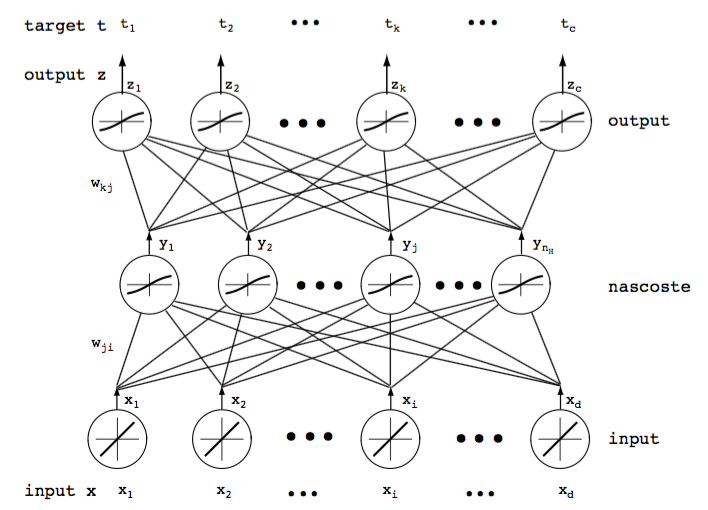
\includegraphics[width=\textwidth]{./notes/immagini/l9-rete.png}
\caption{Esempio di una rete neurale}
\end{figure}

Il cervello umano è sostituito da circa $10^{10}$ neuroni fortemente
interconnessi tra loro (da  $10^{4}$ a  $10^{5}$ connessioni), il tempo di risposta
di un neurone è di circa 0.001 secondi.

Considerando che per riconoscere il contenuto di una scena un umano
impiega circa 0.1 secondi, ne segue che il cervello umano sfrutta
pesantemente il calcolo parallelo: infatti, in questo caso, non più
effettuare più di 100 calcoli seriali.

Questo funzionamento va in contrasto con quello attuale dei nostri
processori, i quali ottengono ottime prestazioni nelle operazioni
seriali ma sono in difficoltà con il calcolo parallelo.

Una rete neurale artificiale è un sistema costituito da unità
interconnesse che calcolano funzioni numeriche, ci sono vari tipi di
unità:

\begin{itemize}

\item
  le unità di input che rappresentano le variabili di ingresso;
\item
  le unità di output che rappresentano le variabili di uscita;
\item
  le unità nascoste che rappresentano le variabili interne che
  codificano (dopo l'apprendimento) le correlazioni tra le variabili di
  input relativamente al valore di output che si vuole generare.
\end{itemize}

Sulle connessioni tra le varie unità sono definiti dei pesi che vengono
definiti dall'algoritmo di apprendimento.

Ci sono due modi per replicare un neurone:

\begin{itemize}
\item Hard-threshold
\item Sigmoidale
\end{itemize}

\subsubsection{Hard-threshold - iperpiano}\label{hard-threshold---iperpiano}

\begin{figure}[htbp]
\centering
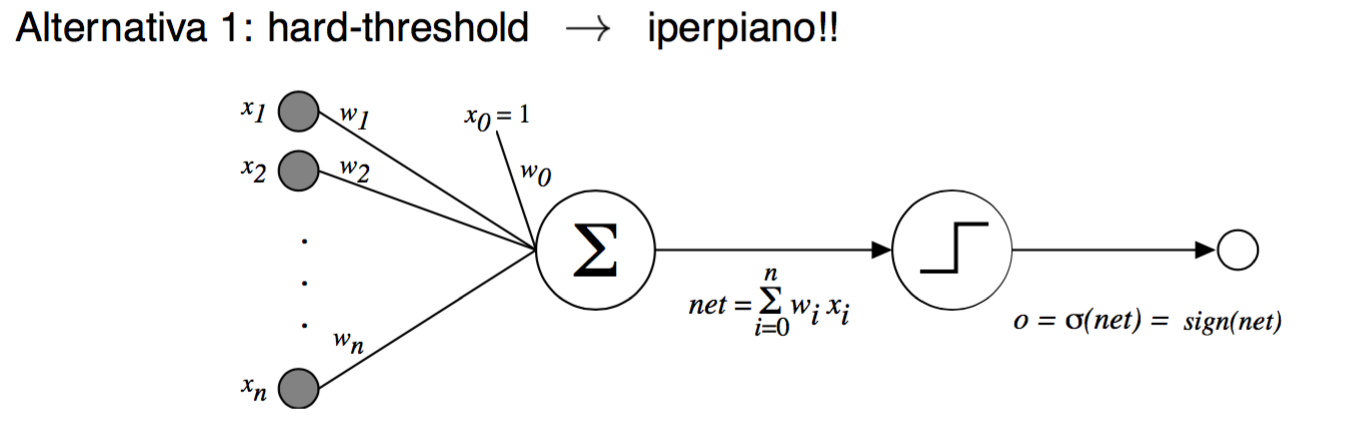
\includegraphics[width=\textwidth]{./notes/immagini/l9-threshold.png}
\caption{Singolo neurone con Hard Threshold. Lo spazio delle ipotesi coincide con quello degli iper-piani in $R^n$.}
\end{figure}

L'idea è quella di avere un vettore di input che rappresenta i nodi di
ingresso da ognuno dei quali arriva un segnale $x_i$. A ogni segnale è
associato un peso $w_i$ che lo amplifica, tutti questi pesi vengono
definiti dall'algoritmo di apprendimento.

Il neurone è poi composto da altri due elementi: il primo che effettua
una sommatoria, detta \textbf{net} di tutti i segnali d'ingresso
moltiplicati per il loro peso, mentre il secondo utilizza il risultato
del primo e calcola una funzione gradino, il cui output è 1 o -1 in base
al segno di net.

Alcune precisazioni:

\begin{itemize}
\item
  Nella sommatoria iniziale gli ingressi vengono rappresentati da $x_1$ a
  $x_n$, ognuno moltiplicato per il proprio peso. Tuttavia è presente anche
  un ingresso $x_0$ sempre fisso a 1, al quale viene associato il peso $w_0$,
  questa componente rappresenta il bias induttivo.
\item
  Possono essere usate altre funzioni gradino oltre a quella del segno.
\end{itemize}

Si può dimostrare che questo tipo di neurone definisce un iper-piano.
Questo perché la sommatoria a partire da \emph{i=1} può essere vista
come un $w^Tx + w_0$ e coincide con la definizione di iper-piano.

\subsubsection{Sigmoidale}\label{sigmoidale}

\begin{figure}[htbp]
\centering
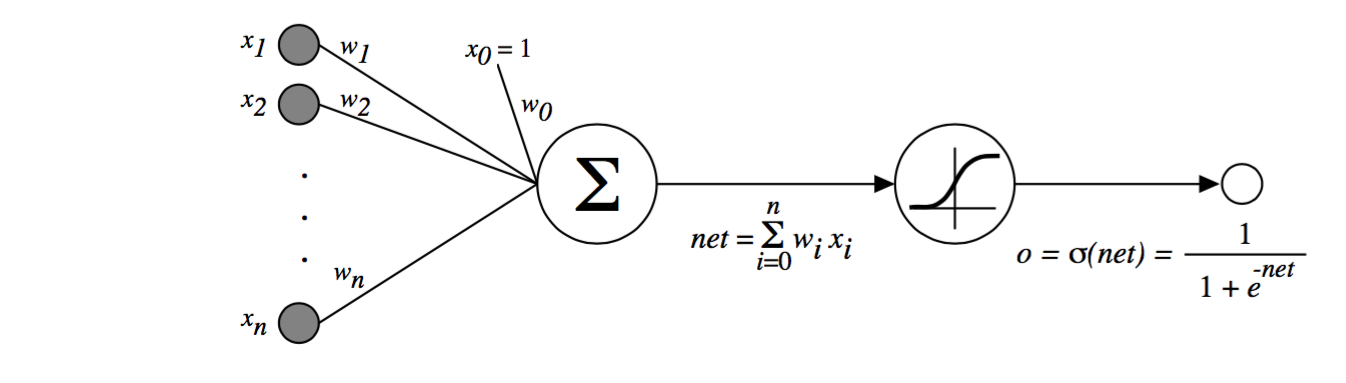
\includegraphics[width=\textwidth]{./notes/immagini/l9-sigmoidale.png}
\caption{Singolo neurone sigmoidale}
\end{figure}

Utilizza la stessa sommatoria \emph{net} alla quale viene applicata la
funzione $\sigma$.

$$
\sigma(z) = \frac{1}{1 + e^{-z}}
$$

La funzione è continua e compresa tra 0 e 1.

Il vantaggio fondamentale di $\sigma$ è che si tratta di una funzione
derivabile e quindi permette di utilizzare l'algoritmo di \textbf{back
propagation}. Un algoritmo che permette di fare apprendimento
all'indietro in grado di funzionare anche su reti composte da più
livelli.

Un'altra caratteristica interessante di questa funzione è che la sua
derivata può essere espressa come una funzione dei valori di input.
Cioè:

$$
\frac{\partial \sigma}{\partial z} = \sigma(z)(1-\sigma(z))
$$

Questa proprietà tornerà utile quando sarà applicato l'algoritmo di back
propagation.

Infine, il neurone sigmoidale può utilizza altre funzioni come la tangente iperbolica, l'unica condizione
è che la derivata della funzione possa essere espressa utilizzando la funzione stessa.

\subsection{Perceptron}\label{perceptron}

È una rete neurale composta da un singolo neurone con Hard Threshold che
viene utilizzata per rappresentare un iper-piano.

L'algoritmo di apprendimento per questa rete cerca dei valori per i vari
pesi $w_i$ in modo da apprendere la funzione target. Per apprendere
i coefficienti corretti vengono utilizzati gli esempi del training set.

\subsubsection{Implementazione di funzioni booleane}\label{implementazione-di-funzioni-booleane}

Ad esempio Percepton può implementare l'operatore \emph{or} con gli
ingressi $\vec{y} \in {0,1}^{n+1}$ (vettori rappresentanti stringhe
binarie), si possono usare come pesi $w_0 = 0.5$ e $w_i = 1$
per $i = 1 \ldots n$.

In modo simile può essere implementato anche l'operatore \emph{and} con
$w_0 = -n+0.5$ e $w_i = 1$ per $i = 1 \ldots n$.

Si può anche realizzare l'operatore \emph{not} con una singola
connessione e con un unico peso negativo.

Un problema che il Perceptron non riesce a risolvere è la \emph{xor},
questo perché si tratta di una funzione non linearmente separabili.

\subsubsection{Apprendimento di funzioni linearmente separabili}\label{apprendimento-di-funzioni-linearmente-separabili}

Si può far apprendere a Perceptron tutte le funzioni linearmente
separabili con un algoritmo che è garantito che termini.

Tuttavia se la funzione da apprendere non è linearmente separabile
l'algoritmo non converge.

Dato un insieme di apprendimento $Tr = {(\vec{x},t)}$ dove $t \in {-1,1}$.

\begin{enumerate}
\item
  Inizializza il vettore dei pesi \emph{w} al vettore nullo (con tutte
  le componenti a 0, possono anche essere random ma piccole)
\item
  Ripeti finché non si raggiunge un punto fisso:

  \begin{enumerate}
  \item
    Seleziona a caso uno degli esempi di apprendimento $(\vec{x},t)$
  \item
    Se $out = sign(\vec{w} \cdot \vec{x}) \neq t$ allora $\vec{w} = \vec{w} + (t - out)\vec{x}$
  \end{enumerate}
\end{enumerate}

Cioè per ogni esempio nel training set va a controllare il segno del
prodotto scalare tra \emph{x} e i pesi, se questo non coincide con il
valore di training è necessario adattare \emph{w} in modo che anche per
\emph{x} venga calcolato il valore corretto.
In questo modo si riesce ad apprendere una funzione che per costruzione
non commette nessun errore nel training set.

L'aggiornamento dei pesi può anche essere espresso considerando i singoli elementi del vettore:

$$
w_i = w_i + (t - out)x_i \qquad \forall i
$$

Nel caso di un neurone sigmoidale, l'apprendimento funziona in modo simile, l'unica differenza è come viene calcolato \textit{out}.